\documentclass{beamer}
\usepackage[orientation=landscape,size=a0,scale=1.4,debug]{beamerposter}
\mode<presentation>{\usetheme{IIT}}
\usepackage{chemformula}
\usepackage[utf8]{inputenc}
\usepackage[english]{babel} % required for rendering German special characters
\usepackage{siunitx} %pretty measurement unit rendering
\usepackage{hyperref} %enable hyperlink for urls
\usepackage{ragged2e}
\usepackage[font=scriptsize,justification=justified]{caption}
\usepackage{array,booktabs,tabularx}
\input{symbols}
\input{mathhdr}
\usepackage{media9}%

\usepackage{graphicx}\graphicspath{{../figures/}} 
% \renewenvironment{thebibliography}[1]{%
%   \section*{\refname}\inparaenum[{[}1{]}]}{\endinparaenum}
% \renewcommand{\bibitem}[1]{\item}

\newcolumntype{Z}{>{\centering\arraybackslash}X} % centered tabularx columns
\sisetup{per=frac,fraction=sfrac}
%ICRA
% \title{\huge Whole-body Trajectory Optimization for Non-periodic Dynamic Motions on Quadrupedal Systems}
%Workshop
\title{\huge Trajectory Optimization and Dynamic Walking Adaptation\\ for Rough Terrain Locomotion}
\author{Andreea Radulescu$^{1}$, Ioannis Havoutis$^{2,3}$, Darwin G. Caldwell$^1$, Claudio Semini$^{1}$}
\institute[]{$^{1}$Dynamic Legged Systems Lab., Department of Advanced Robotics, Istituto Italiano di Tecnologia, Genova, Italy\\ 
$^{2}$Robot Learning and Interaction Group, Idiap Research Institute, Martigny, Switzerland \\
$^{3}$Oxford Robotics Institute, Department of Engineering Science, University of Oxford, United Kingdom}
\date{\today}

% edit this depending on how tall your header is. We should make this scaling automatic :-/
\newlength{\columnheight}
\setlength{\columnheight}{65cm}

\begin{document}
\begin{frame}
\begin{columns}
  \begin{column}{.29\textwidth}
  
\begin{beamercolorbox}[center]{postercolumn}
\begin{minipage}{.98\textwidth}  % tweaks the width, makes a new \textwidth
\parbox[t][\columnheight]{\textwidth}{ % must be some better way to set the the height, width and textwidth simultaneously
\begin{myblock}{Introduction}
\textbf{We present a whole-body optimization methodology for non-periodic tasks on quadrupedal systems. 
This approach delivers solutions involving multiple contacts without 
the need for predefined feet placements.}
\vspace*{10mm} 

Autonomous legged robots will need to handle a wide range of tasks 
in complex environments. Biological legged systems can achieve a variety of whole body movements, in order to manipulate
and traverse their environment. 

\begin{center}
% \movie[height = 0.6\textwidth, width = 0.8\textwidth, poster, showcontrols]{}{Movies/trimmed_poseRec_ICRA17.mp4}
% \includemovie{.85\textheight}{.85\textheight}{Movies/trimmed_poseRec_ICRA17.flv}%
\begin{columns}
\column{.46\textwidth}
\begin{center}
\includemedia[ width=\linewidth, activate=pagevisible, deactivate=onclick,
  addresource=Movies/goat_parkour.m4v,
  flashvars={source=Movies/goat_parkour.m4v
  &loop=true
  &autoPlay=true}]
  {{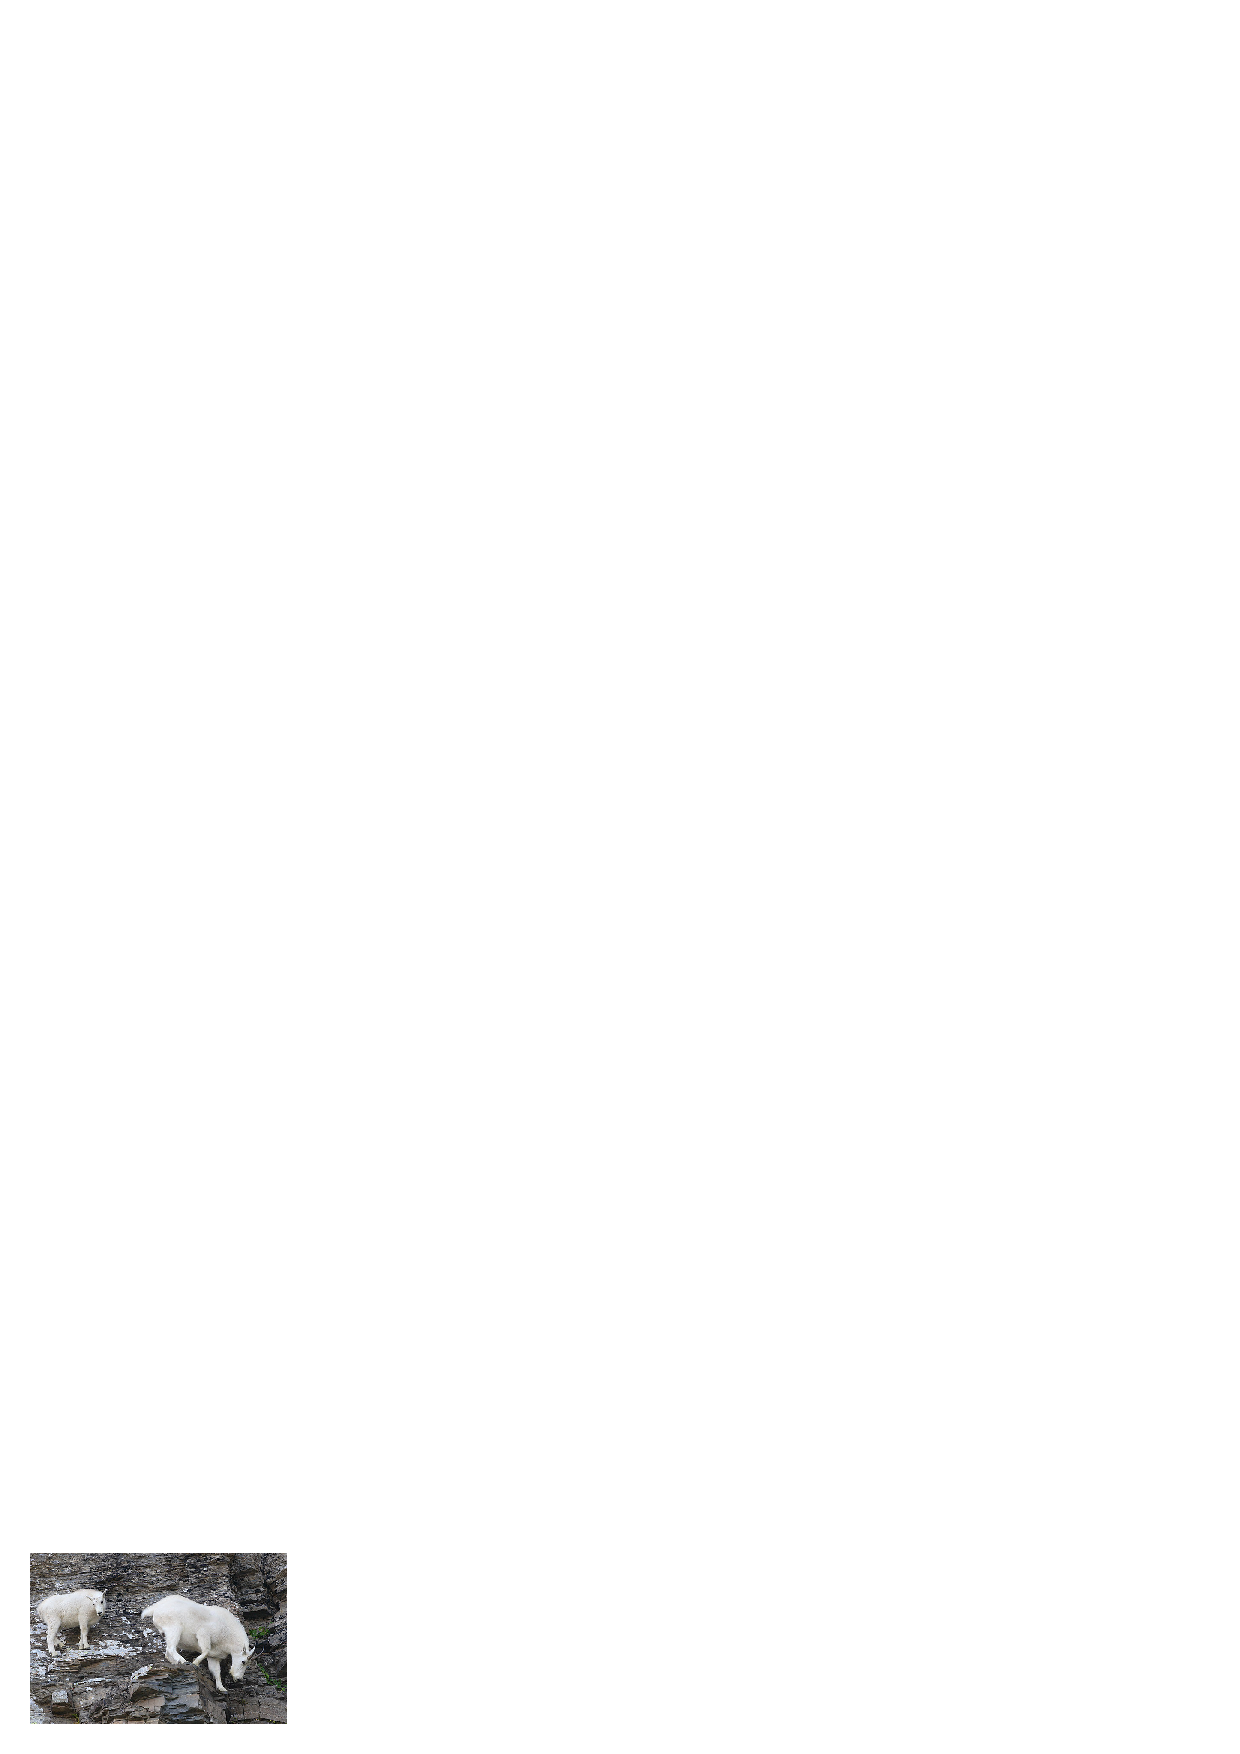
\includegraphics[width=\linewidth]{mountaingoat.jpg}}}{/home/andreea/media9/players/VPlayer9.swf}
\end{center}   
\column{.54\textwidth} 
\begin{center}
\includemedia[ width=\linewidth, activate=pagevisible, deactivate=onclick,
  addresource=Movies/dog_parkour_short.m4v,
  flashvars={source=Movies/dog_parkour_short.m4v
  &loop=true
  &autoPlay=true}]
  {{\includegraphics[width=\linewidth]{parkour_dog.jpg}}}{/home/andreea/media9/players/VPlayer9.swf} 
\end{center}   
\end{columns}
  
\end{center} 
\vspace*{3mm}

When transferring these skills to their robotic counterparts,
most research has focused on periodic tasks (in complex environments
teleoperation or predefined heuristics are frequently used).
\vspace*{5mm}

Various optimization approaches were proposed for dealing with multiple contact events. 
Recently, the Covariance Matrix Adaptation (CMA) algorithm \cite{hansen2001completely} 
was used to generate whole body movements for both periodic and non-periodic tasks \cite{shafii2015learning,
gehring2016practice}.
% We employ a realistic 
% simulation of the hydraulically actuated HyQ2Max quadrupedal system for 
% investigations on two distinctive tasks: rearing and posture recovery. 
% We present a whole-body optimization methodology for non-periodic tasks on quadrupedal systems. 
% This approach delivers solutions involving multiple contacts without 
% the need for predefined feet placements. 
% The results obtained show the potential of optimization approaches for 
% motion synthesis in the context of complex tasks.
\end{myblock}


\begin{myblock}{Our Methodology}
\vspace*{5mm}

\begin{center}
 \textbf{A. Robot description and System model}\\
\end{center}

\begin{columns}
\column{.55\textwidth}
We use a realistic simulation of the 80 kg HyQ2Max \cite{semini16tmech} 
quadrupedal robotic system with contacts. 
% \vspace*{5mm}

Each limb has 3 actuators:\\
\begin{itemize}
 \item HAA (hip abduction/adduction)
 \item HFE (hip flexion/extension)
 \item KFE (knee flexion/extension)
\end{itemize}
% HAA (hip abduction/adduction), HFE (hip flexion/extension) and KFE (knee 
% flexion/extension). 

\column{.45\textwidth}
 \begin{figure}
  \centering
  \includegraphics[width=0.9\textwidth]{hyq2max_cad.jpg}
 \end{figure}
\end{columns}
\vspace*{5mm}
We model the behavior of the platform as a rigid body system:
\begin{equation}
\bM \left( \bq \right) \ddot{\bq} + \bC \left( \bq, \dot{\bq} \right) \dot{\bq}+ 
\bg \left( \bq \right) + \bD \dot{\bq} = \bJ^T_{c} \lambda \left( \bq, 
\dot{\bq} \right) + \bS^{T} \btau,
\label{eq_motion_general}
\end{equation}
\noindent 
with: $\bq = \left[\bq_{B}, \bx_{B}, \bq_{J} \right]^{T}$,
$ \bx = \left[  \bq ,   \dot{\bq} \right] ^{T} =
 \left[ \bq_{B}, \bx_{B}, \bq_{J}, \dot{\bq_{B}}, 
\dot{\bx_{B}}, \dot{\bq_{J}} \right] ^{T}$.
% \begin{equation}
%  \bq = \left[\bq_{B}, \bx_{B}, \bq_{J} \right]^{T} 
% \end{equation}
% 
% \begin{equation}
%  \bx = \left[  \bq ,   \dot{\bq} \right] ^{T} =
%  \left[ \bq_{B}, \bx_{B}, \bq_{J}, \dot{\bq_{B}}, 
% \dot{\bx_{B}}, \dot{\bq_{J}} \right] ^{T}
%  \label{eq_state}
% \end{equation} 
\vspace*{2mm}
\begin{center}
 \begin{tabular}{c | c} 
 $\bq_{B}$ & COM orientation ($RPY$)\\  
 \hline
 $\bx_{B}$ & COM position ($XYZ$)\\ 
 \hline
 $\bq_{J}$ & joint angles \\
\end{tabular}
\end{center}

\end{myblock}\vfill
}\end{minipage}\end{beamercolorbox}
\end{column}
	
\begin{column}{.3\textwidth}
\begin{beamercolorbox}[center]{postercolumn}
\begin{minipage}{.98\textwidth}  % tweaks the width, makes a new \textwidth
\parbox[t][\columnheight]{\textwidth}{ % must be some better way to set the the height, width and textwidth simultaneously
\begin{myblock}{Our Methodology}


% 
\begin{center}
 \textbf{B. Optimization}\\
\end{center}


We employ a CMA Exploration Strategy based approach to address dynamic non-periodic tasks.
% This technique proved effective in handling nonlinear, high-dimensional problems. 
% The method operates by generating and evaluating 
% a set of solutions at each iteration. The samples are extracted from a 
% multivariate Gaussian distribution. After their evaluation 
% the covariance matrix of the search distribution is adapted. 
% As this is a local 
% minimizer, an initial guess for the solution is provided at the start. 
% 
% For complex robotic systems such as HyQ2Max, the main challenge consists of 
% determining the suitable joint motions which achieve the desired movement for 
% each given task. Using a direct optimization approach on the time-parametrized joint or torque trajectories would involve an inconveniently large search 
% space. Hence, we 
We use a parametrized policy to encode joint position/torque profiles, represented as 
a weighted average of Gaussian kernels\footnote{We use 12 policies, one for each joint, $M=16$ Gaussian kernels, means equally spaced, $\sigma^2 = 0.01$}: 
\begin{equation}
 \label{weighted_sum}
 f(t) = \sum_{i=1}^{M} w_i \phi_i(t)/ \sum_{i=1}^{M} \phi_i(t), \;  \phi_i(t) = exp(- \frac{1}{2 \sigma^2} (t-\mu_i))
 \end{equation}
where $w_i$ are the weights associated with each kernel $\phi_i, \; i \in [1, M]$, defined by mean $\mu_i$ and 
variance $\sigma^2$.
% as in:
% \begin{equation}
%  \phi_i(t) = exp(- \frac{1}{2 \sigma^2} (t-\mu_i)).
%  \label{gaus_kernels}
% \end{equation}
% 

\begin{figure}[h!]
  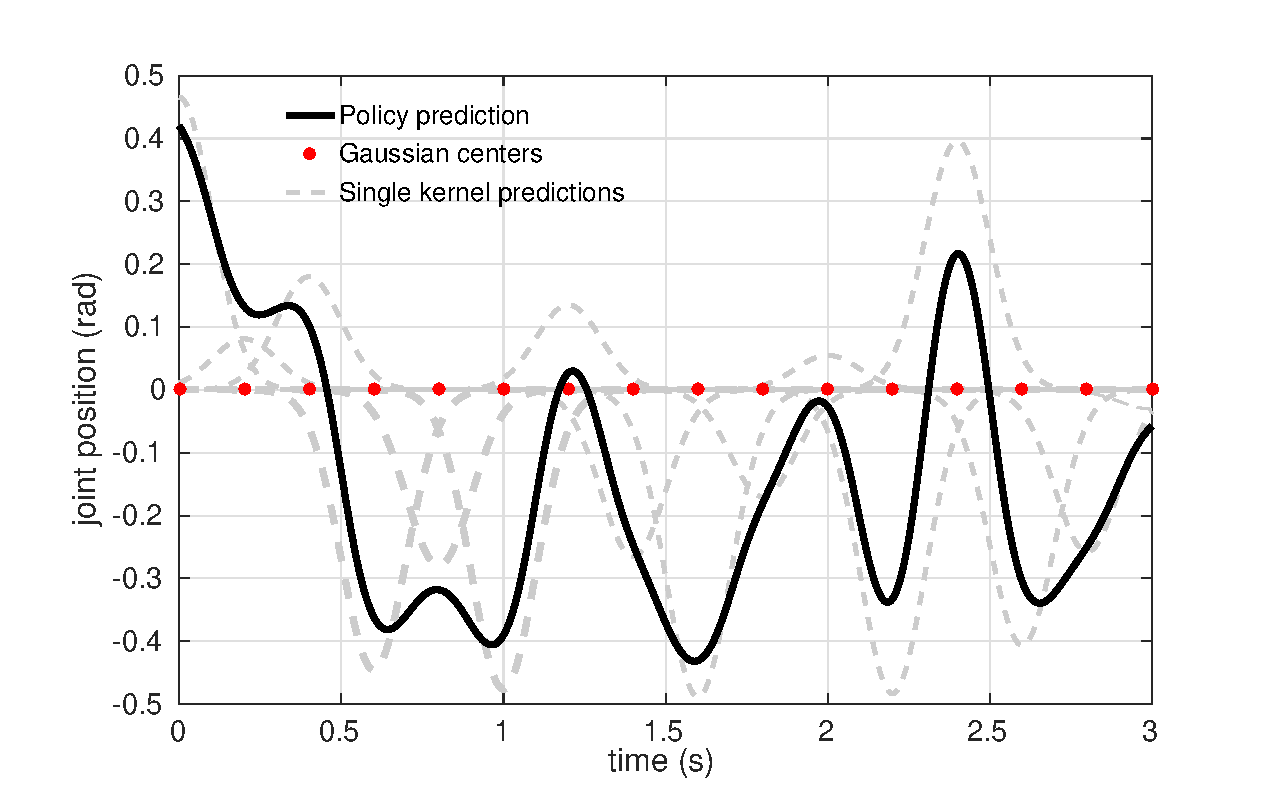
\includegraphics[scale=1]{example_gr2.eps} 
\end{figure}
    
The CMA algorithm is used to optimize the weights of all 
policies according to a task specific cost function (\ref{eq:cost_general}), applied to the 
whole body trajectory generated through (\ref{weighted_sum}) : 
\begin{equation}
 \label{eq:cost_general}
  J = p (\mathbf{s}_T, \mathbf{\dot{s}}_T)+\int^{T}_{t=0}\rc(\mathbf{\tau}_t, \bq_{J})\;\dt, \; t \in [0,T]
\end{equation}
\noindent
where $\mathbf{s}_t = [\bq_{B}, \bx_{B}]'$ is the trunk state
and $\btau_t$ is the set of 12 torque actuation commands at time $t \in 
[0,T]$.


The running cost $ \rc $ seeks 
to minimize the effort used for producing the motion:
\begin{eqnarray}
 \label{eq:final_cost1}
  \rc( \mathbf{s}_t, \mathbf{\dot{s}}_t, \mathbf{\tau}_t)  & = & Q_{3}  {\mathbf{\tau}_t}^{2} 
    + Q_{6} [(\bq_{J} - {\bq_{J}}_{max}))^2 \Big|_{\bq_{J}  > {\bq_{J}}_{max}} \\ \nonumber
    & + & (\bq_{J} - {\bq_{J}}_{min}))^2 \Big|_{\bq_{J}  < {\bq_{J}}_{min}}] 
\end{eqnarray}
The final cost $p$ evaluates the success of the motion according to the goals 
(desired final states ($\bq^{*}_{B}, \bx^{*}_{B}$)):
\begin{eqnarray}
 \label{eq:final_cost}
%   \rc( \mathbf{s}_t, \mathbf{\dot{s}}_t, \mathbf{\tau}_t)  & = & Q_{3}  {\mathbf{\tau}_t}^{2} 
%     + Q_{6} [(\bq_{J} - {\bq_{J}}_{max}))^2 \Big|_{\bq_{J}  > {\bq_{J}}_{max}} \\ \nonumber
%     & + & (\bq_{J} - {\bq_{J}}_{min}))^2 \Big|_{\bq_{J}  < {\bq_{J}}_{min}}] \\ \nonumber
  p (\mathbf{s}_T, \mathbf{\dot{s}}_T) & = & (\bq_{B}(T) - \bq^{*}_{B})' Q_{1} (\bq_{B}(T) - \bq^{*}_{B}) \\ \nonumber
  & + & (\bx_{B}(T) - \bx^{*}_{B})' Q_{2} (\bx_{B}(T) - \bx^{*}_{B})
\end{eqnarray}
\noindent
where ${\bq_{J}}_{min},\; {\bq_{J}}_{max}$ are the upper and lower bounds on the joint limits $\bq_{J}$,
and $Q_{i}, \; i \in \{1,2,3,4\}$ are the relative weights associated with the terms for each individual task.
% 
% 
% Since the CMA-ES is a local method, a starting policy is required.
% In our experiments the policies are initialized with values that maintain an 
% initial pose (in the case of rearing tasks) or as a direct interpolation 
% between the initial configuration and desired final pose (for posture recovery).
% No specific footstep sequence information is enforced. We apply 
% a staged optimization approach, where preliminary solutions are obtained using 
% a relaxed cost (e.g., lower weights for the joint limits term). The complexity of the cost 
% function is increased gradually, until the solution meets all the desired 
% requirements\footnote{We note that the robot model used incorporates a model of the
% actuator dynamics, thus increasing the feasibility of the resultant behavior.}. The procedure
% is based on optimization techniques, but the policy always starts from a general
% non-specific point. Thus, the method can be viewed as a learning approach, where a
% strategy is learned from scratch, rather than an existing solution is improved.
% 
% An example of such a resultant policy is depicted in Fig. \ref{fig:policy_example} where the $M=16$ Gaussian kernels'
% means are equally spaced, the variances $\sigma^2$ are all fixed to $0.01$ and 
% the weights $w_i$ have been sampled from the interval $[-1,1]$. In our experiments we use 12 such representations, one for each degree
% of freedom (DoF) of the quadrupedal system.
% 
% \begin{figure}[t!]
%  \centering
%  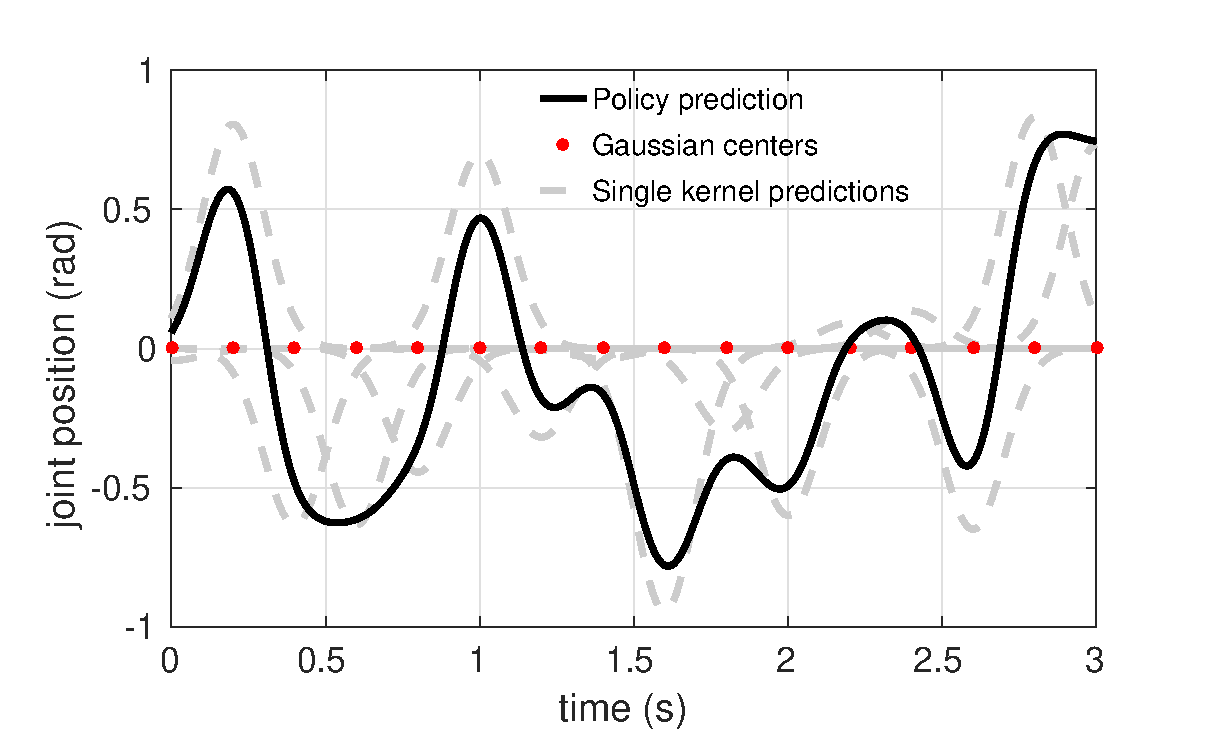
\includegraphics[scale=.4]{example_gr3.eps} 
%  \caption{Example of a policy encoded as a weighted average of 
%  Gaussian kernels: the means $\mu_i$ are equally spaced and the 
%  variances are all fixed to $0.01$ and the weights have been 
%  sampled from $[-1,1]$.}
%  \vspace*{-5mm}
%   \label{fig:policy_example}
% \end{figure}


\end{myblock}\vfill
}\end{minipage}\end{beamercolorbox}
\end{column}

\begin{column}{.4\textwidth}
	\begin{beamercolorbox}[center]{postercolumn}
	\begin{minipage}{.98\textwidth} % tweaks the width, makes a new \textwidth
	\parbox[t][\columnheight]{\textwidth}{ % must be some better way to set the the height, width and textwidth simultaneously
	\begin{myblock}{Results}
	
	\begin{columns}
	
	\column{.5\textwidth}
	\begin{center}
	\textbf{A. Rearing}\\
	\vspace*{5mm}
	\end{center}
	$\bq^{*}_{B}= (-, \pi/3 , -)rad$, $\bx^{*}_{B}= (-,-, 0.9)m$ 
	$Q_{1} = 10^3, \; Q_{2} = 10^2, \; Q_{3} = 0.1, \; Q_{4} = 1$
	
	\begin{figure}[h!]
	  \centering
% 	  \vspace*{+4mm}
% 	  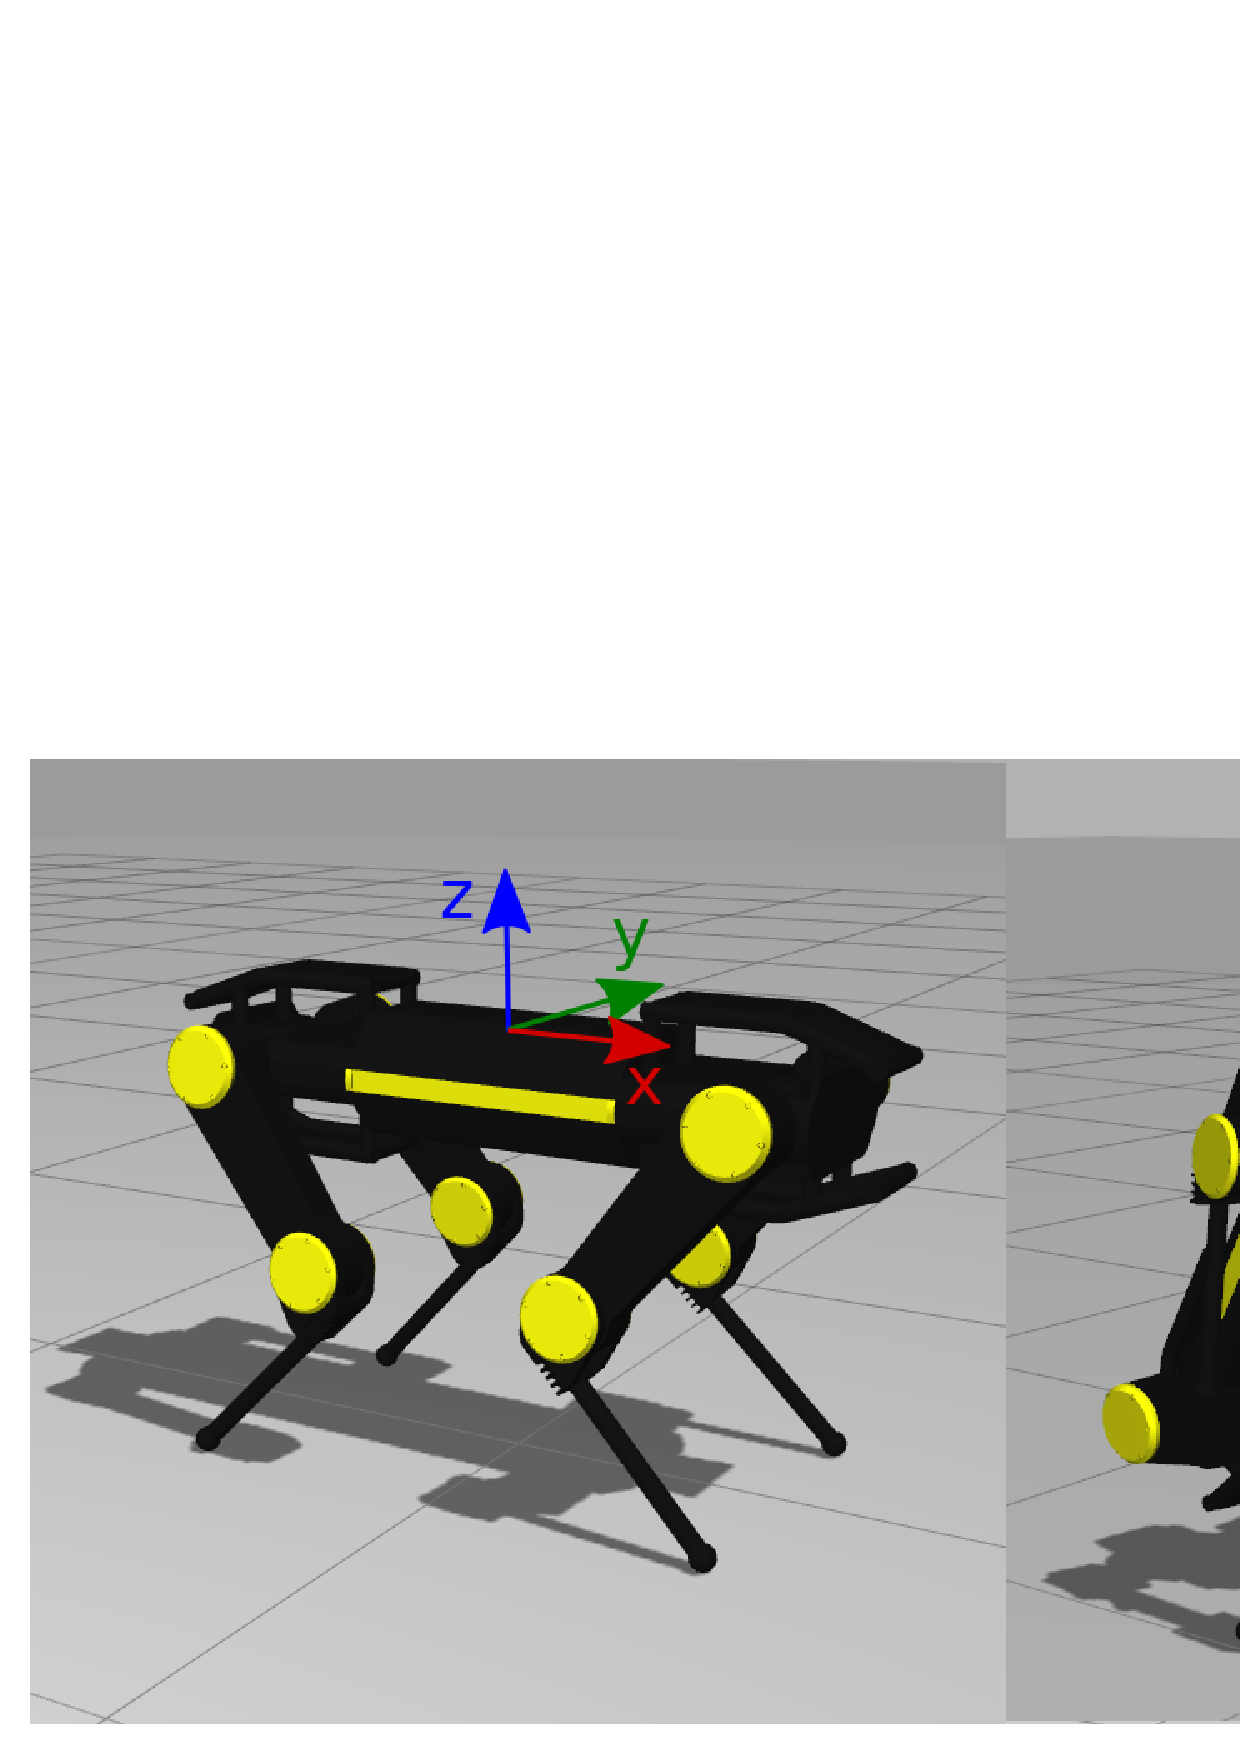
\includegraphics[width=\linewidth]{rearing_befor_after_ins.png}\\
\includemedia[
  width=\linewidth,
%   height=0.25\linewidth,
  activate=onclick,
  deactivate=onclick,
  addresource=Movies/RearingExplore_25May_3.m4v,
  flashvars={source=Movies/RearingExplore_25May_3.m4v
%   &loop=true
%   &autoPlay=true
  }]
  {{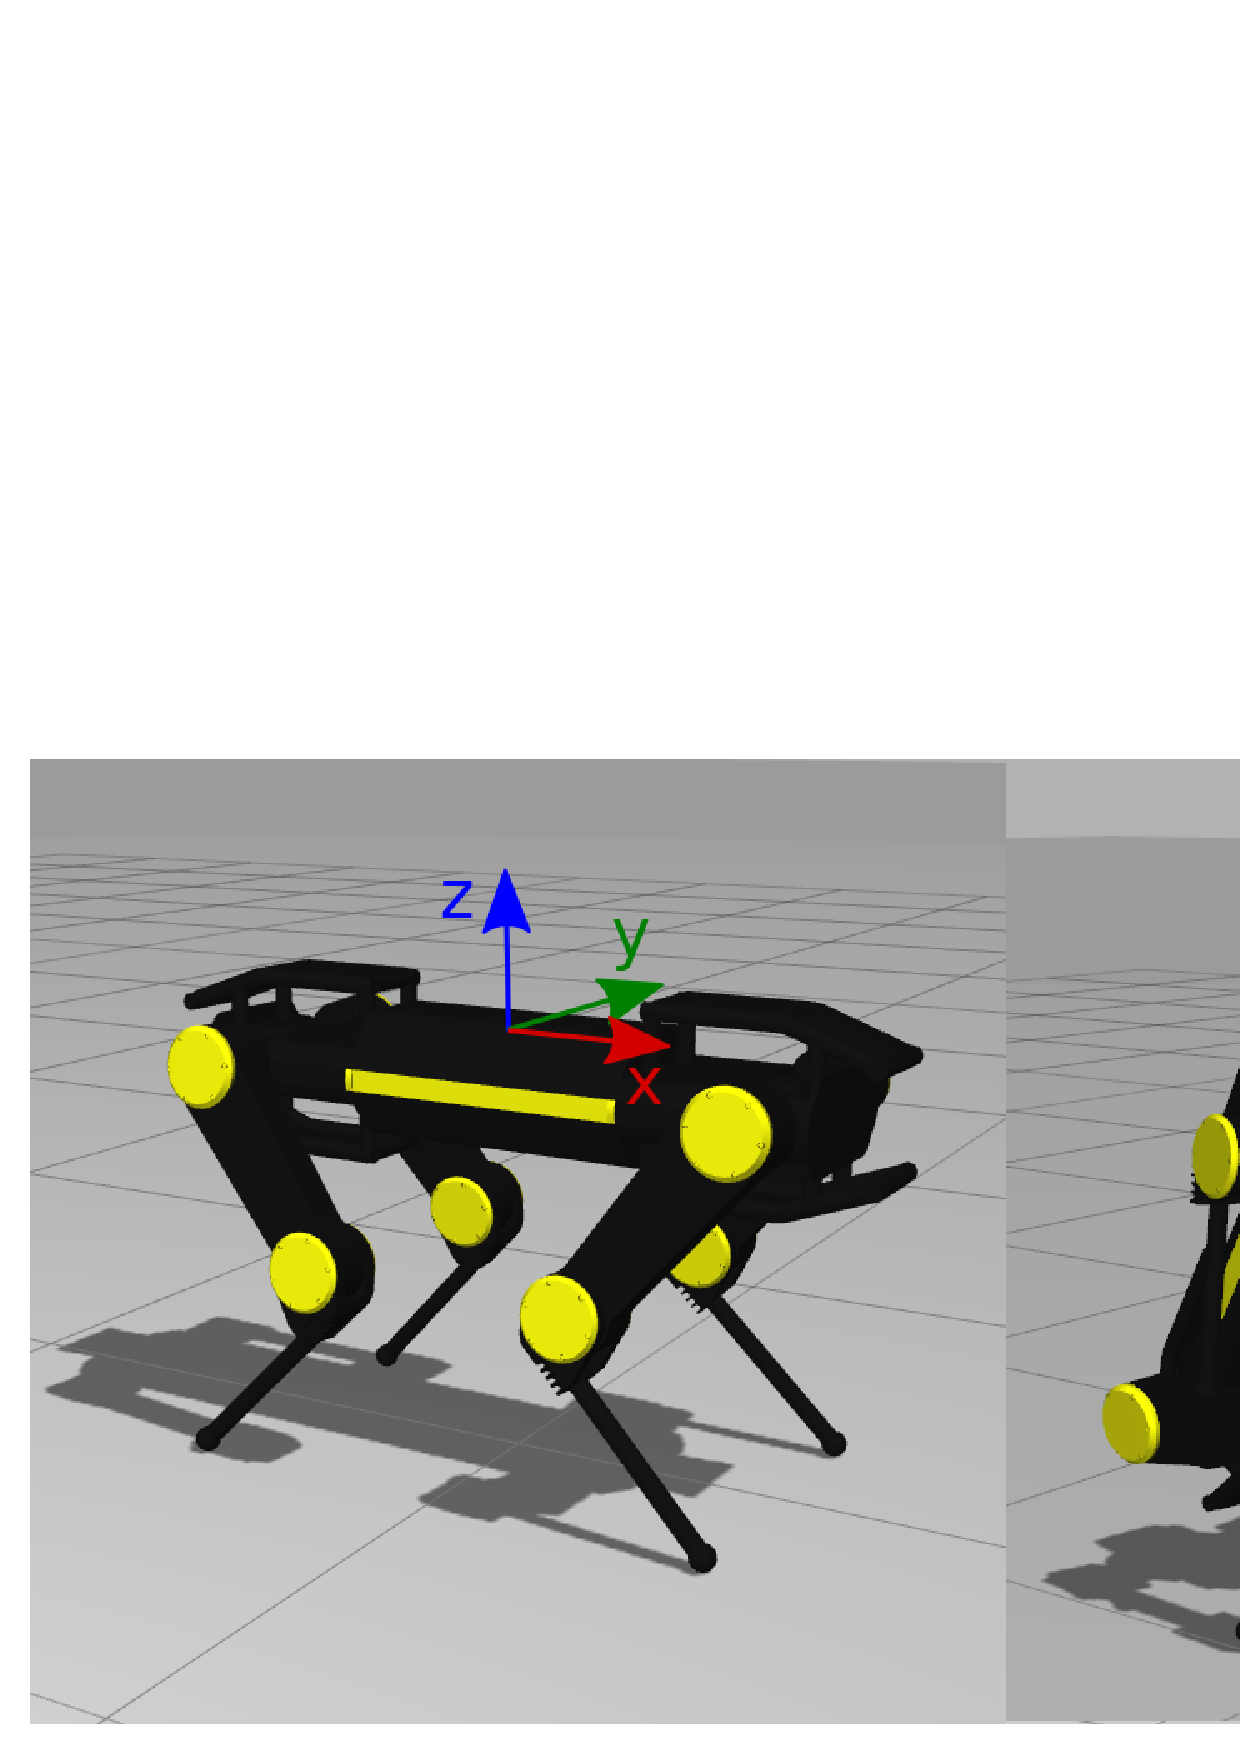
\includegraphics[width=\linewidth]{rearing_befor_after_ins.png}}}{/home/andreea/media9/players/VPlayer9.swf}\\
	  \vspace*{3mm}
	  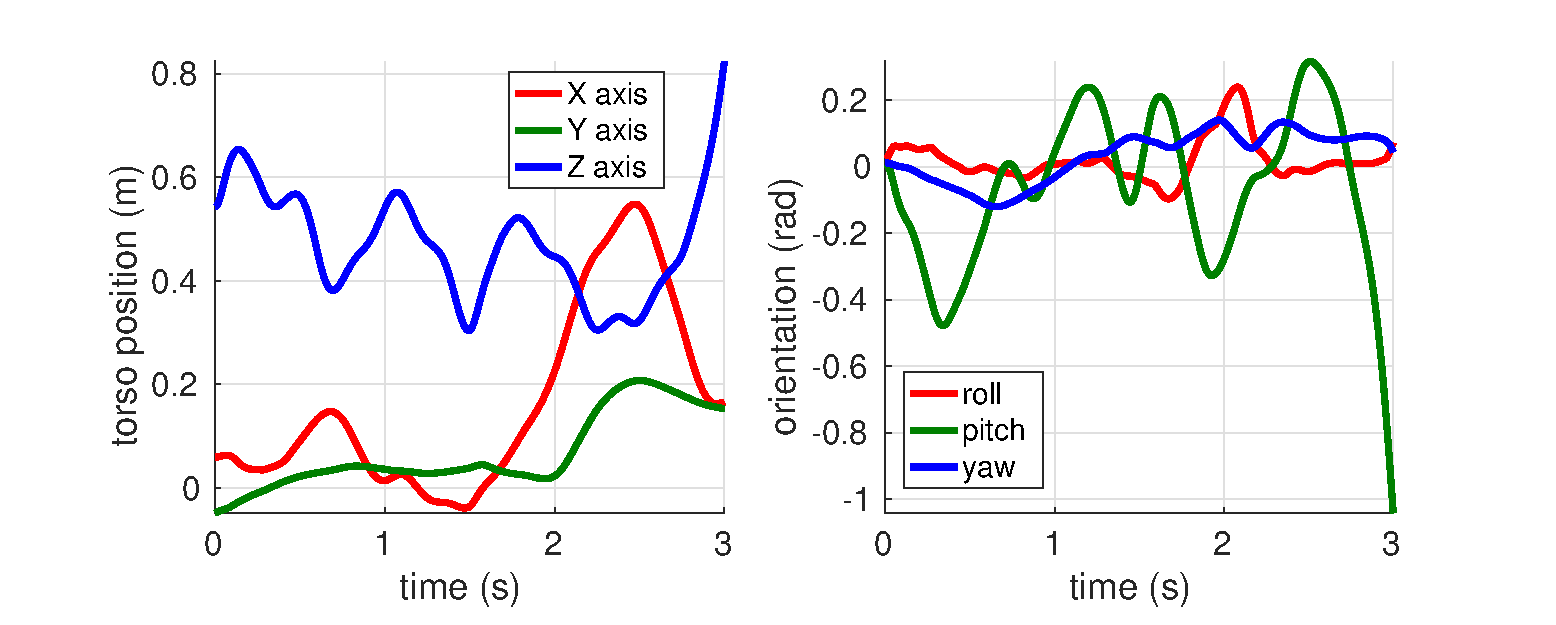
\includegraphics[width=\linewidth]{PRec_solution_joints_1_ICRA.eps} \\
	  \vspace*{3mm}
	  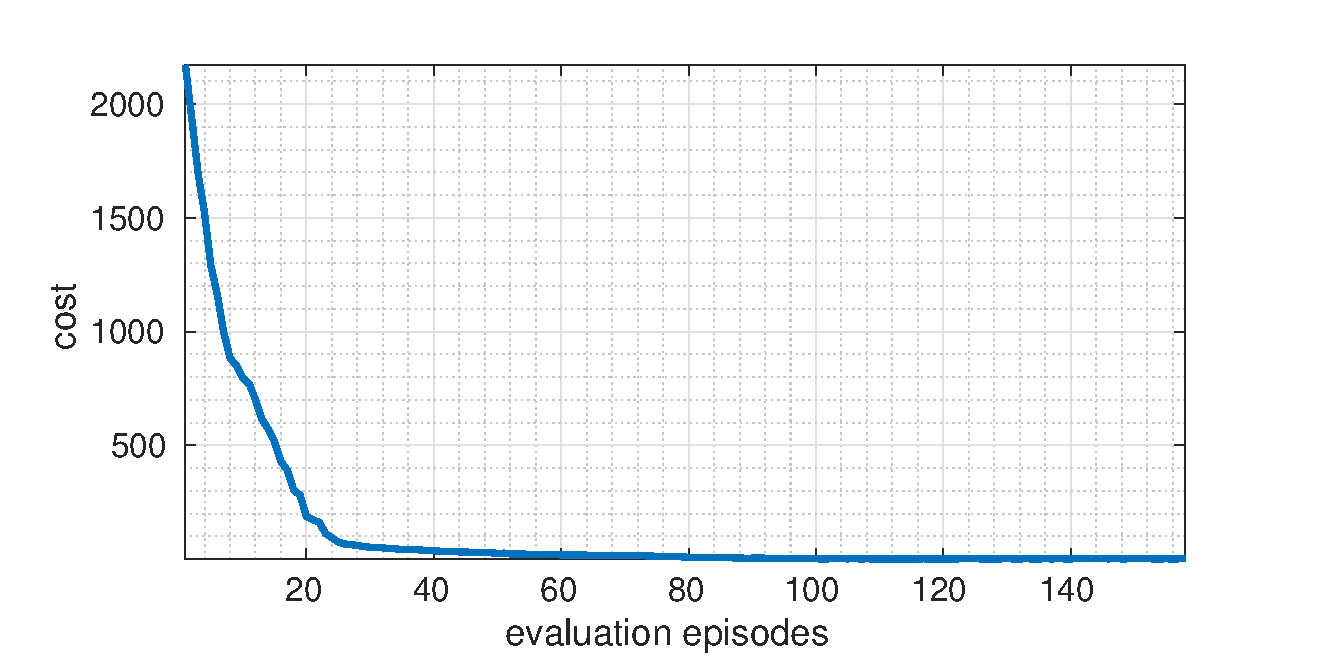
\includegraphics[width=\linewidth]{PRec_solution_1_ICRA.eps}
% 	   \caption{(a) HyQ2Max performing the rearing task in simulation under the resultant 
% 	    policy. \textit{Left:} initial pose.\textit{Right:} final pose.
% 	    (a) Evolution of the cost for the rearing experiment ($158$ evaluation episodes with $19$ samples per episode). }
	   \label{fig:rearing_behaviour}
	\end{figure}
	
	\column{.5\textwidth}
	\begin{center}
	\textbf{B. Pose recovery}\\
	\vspace*{5mm}
	\end{center}
	\vspace*{-4mm}
	$\bq^{*}_{B}= (0,0,0)rad$, $\bx^{*}_{B}= (-,-, 0.61)m$ 
	$Q_{1} = 10^3, \; Q_{2} = 10^3, \; Q_{3} = 0.1, \; Q_{4} = 1$.
	\begin{center}
	 \includemedia[
	  width=\linewidth, activate=pagevisible, deactivate=onclick,
	  addresource=Movies/trimmed_poseRec_ICRA17.mp4,
	  flashvars={source=Movies/trimmed_poseRec_ICRA17.mp4
	  &loop=true
	  &autoPlay=true}]
	{{\includegraphics[width=\linewidth]{sr_after.png}}}{/home/andreea/media9/players/VPlayer9.swf}
	\end{center}

	\begin{figure}[t!]
	\centering
% 	  \vspace*{+4mm}
% 	  \includegraphics[width=\linewidth]{sr_after.png}\\
	  \vspace*{-5mm}
	  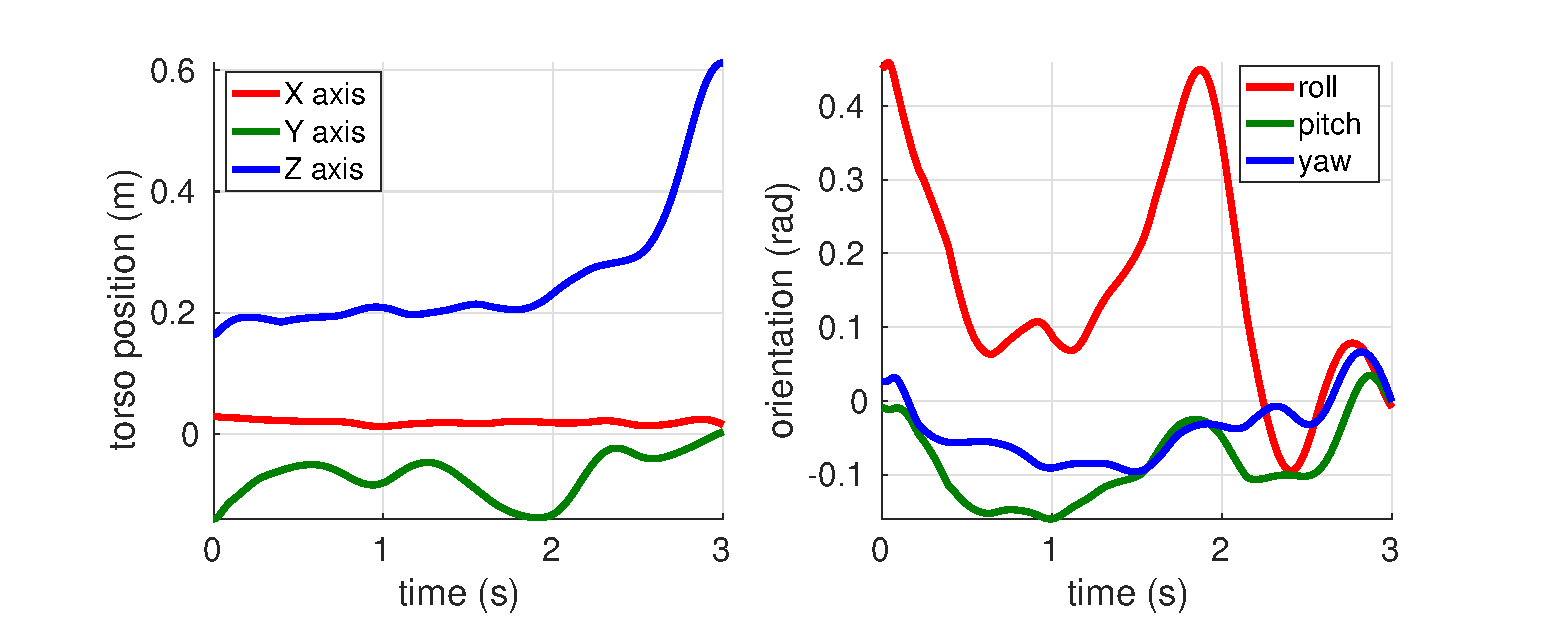
\includegraphics[width=\linewidth]{sr_solution_1_ICRA.eps} \\
	  \vspace*{3mm}
	  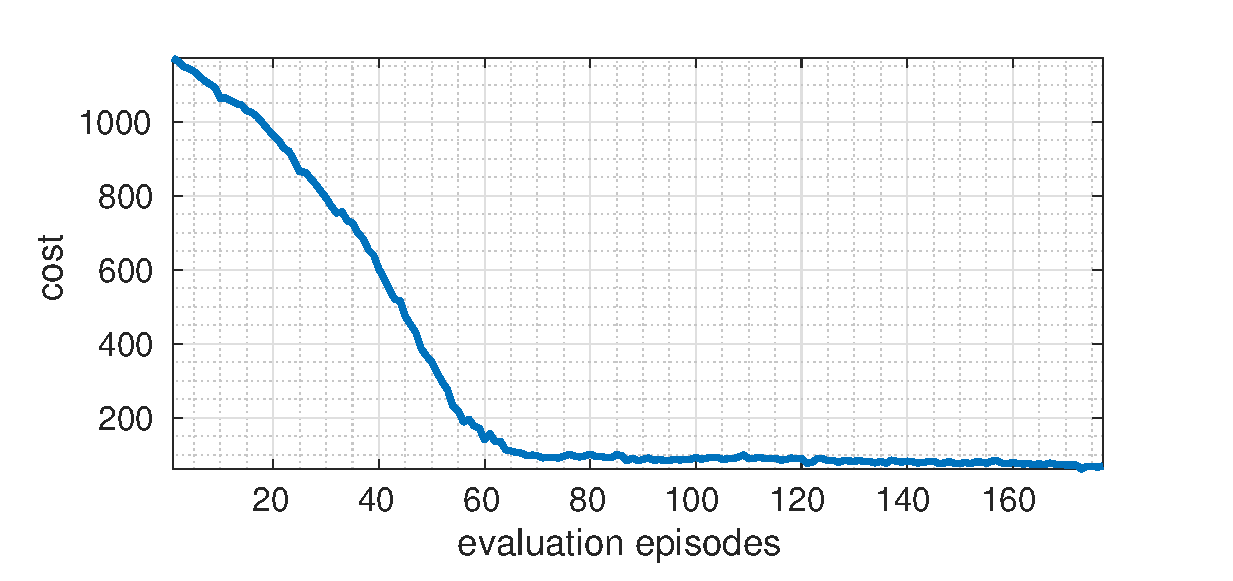
\includegraphics[width=\linewidth, height=0.155\textheight]{sr_cost_1_ICRA.eps}
	\label{fig:sr_behaviour}
	\end{figure}	
	
	\end{columns}
	

	

% 	\vspace*{5mm}
% 	\begin{figure}[h!]
% 	\centering
% % 	  \vspace*{+4mm}
% 	  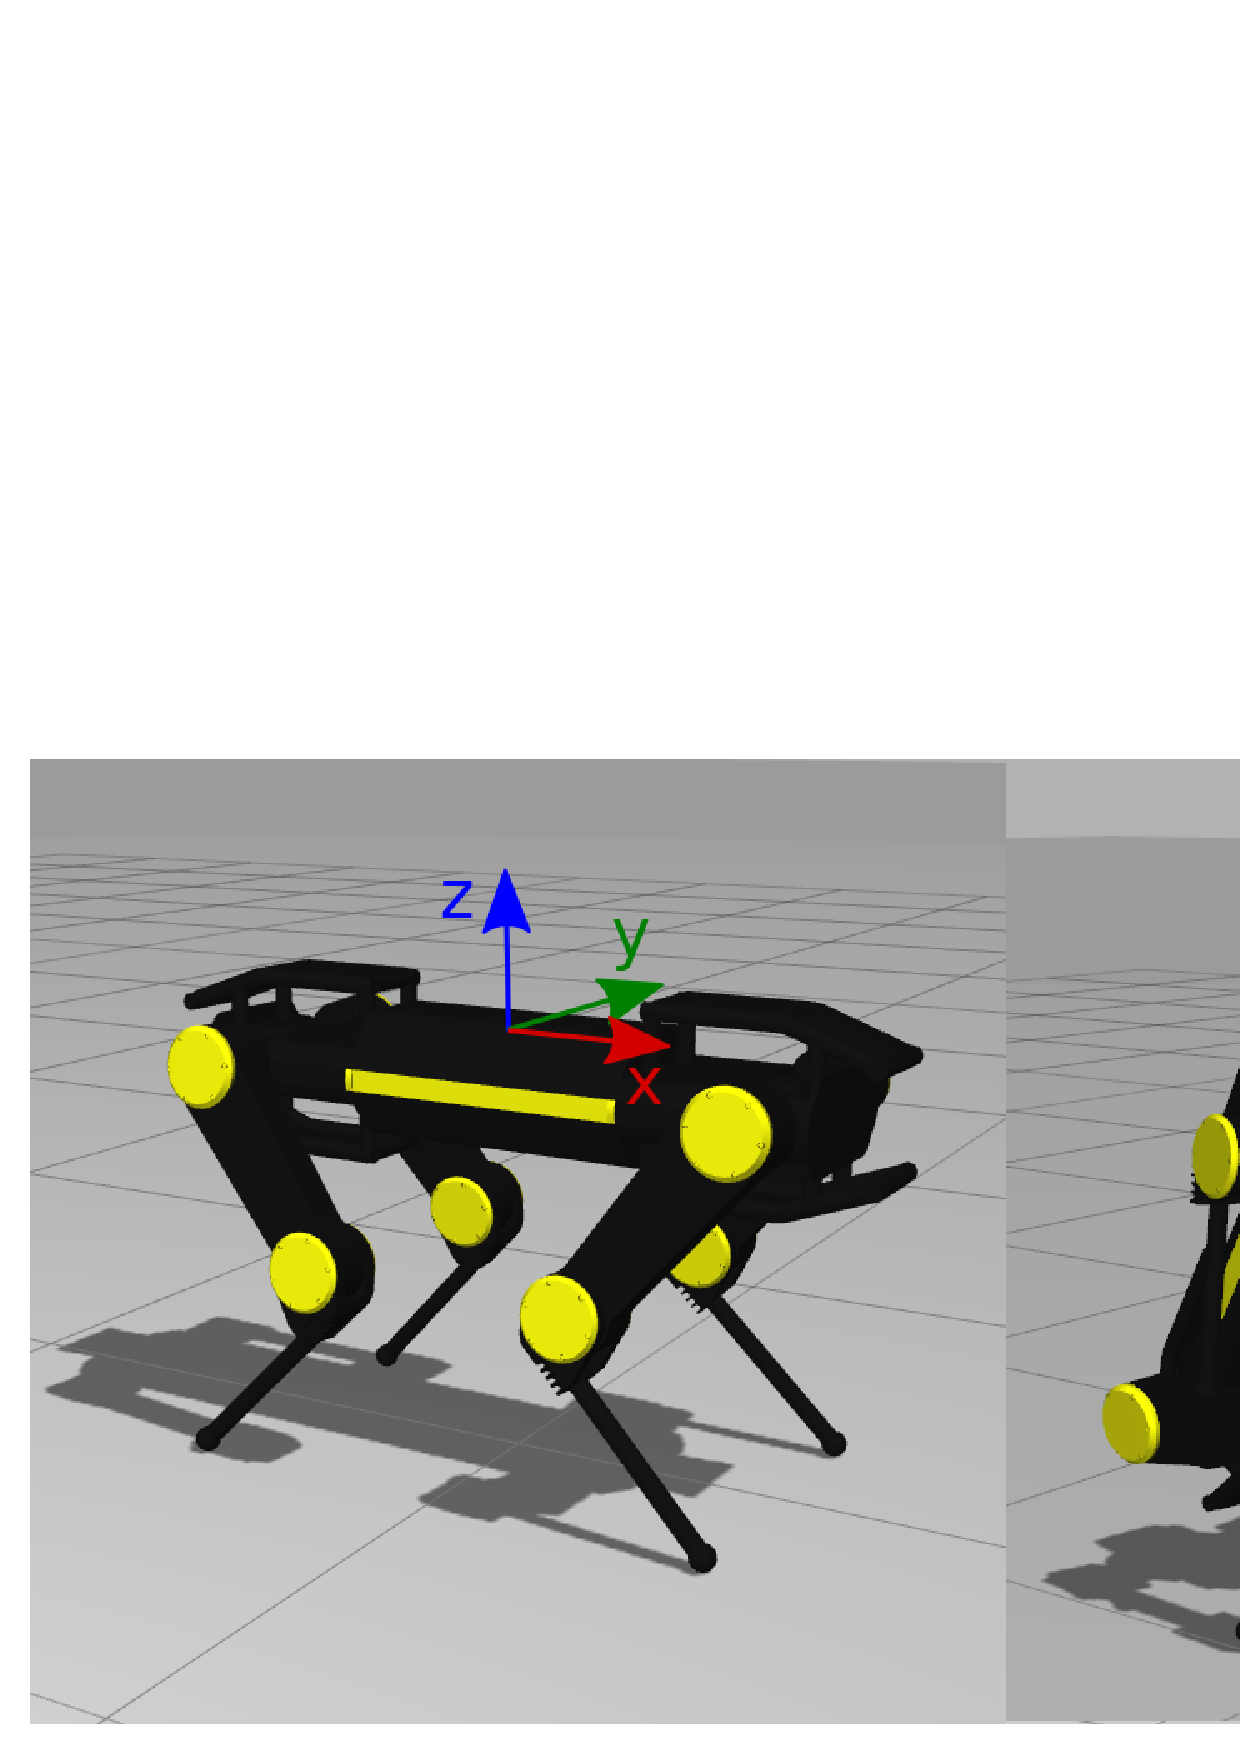
\includegraphics[scale=.45]{rearing_befor_after_ins.png} 
% % 	  \hspace*{5mm}
% 	  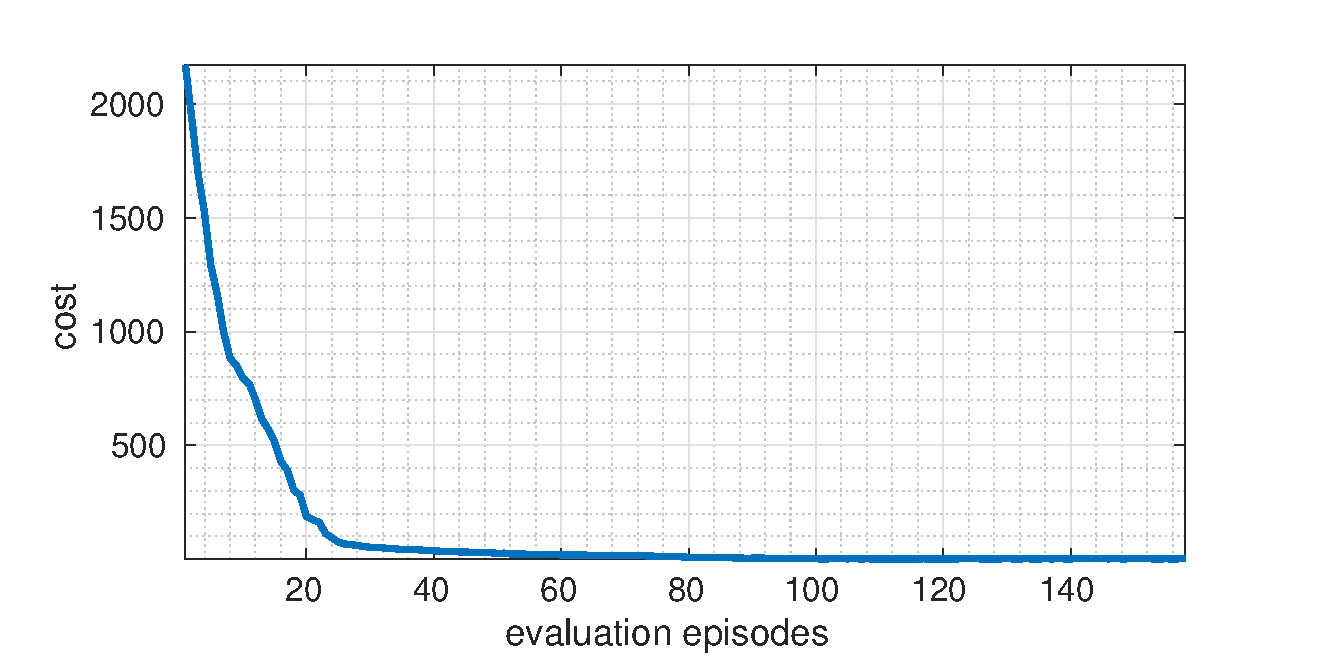
\includegraphics[scale=.75]{PRec_solution_1_ICRA.eps}
% % 	   \caption{(a) HyQ2Max performing the rearing task in simulation under the resultant 
% % 	    policy. \textit{Left:} initial pose.\textit{Right:} final pose.
% % 	    (a) Evolution of the cost for the rearing experiment ($158$ evaluation episodes with $19$ samples per episode). }
% 	   \label{fig:rearing_behaviour}
% 	\end{figure}



	\end{myblock}\vfill
	
	\begin{myblock}{Conclusions \& Future directions}
	 We show a \textbf{whole body optimization approach} for \textbf{non-periodic 
	dynamic movements} on quadrupedal systems. We deliver trajectory solutions which
	involve \textbf{multiple contacts, without any predefined feet placement heuristics}. 
	\vspace*{4mm}
	
	Future work will address: incorporating real-time sensory information from the environment, 
	automatic goal decision and improving the computation speed. We will also tackle 
	hardware validation and expanding the range of tasks.
	\end{myblock}\vfill

	
	\begin{myblock}{References}
		\footnotesize
		\bibliographystyle{ieeetr}
		\bibliography{./icra17radulescu_poster}
	\end{myblock}\vfill
	}\end{minipage}\end{beamercolorbox}
	\end{column}
\end{columns}
\end{frame}
\end{document}
